\section{Deep Learning Architectures \label{archi}}
    % Model descriptions
    \subsection{Deep Learning to Predict Molecular Weight from SMILES}
        \begin{itemize}
            \item The first model we will discuss is a DL model that receives an embedded SMILES string as input and as a result returns its prediction of the molecular weight. This model is shown in Figure \ref{fig:mw-architecture}.
            \item Its architecture consisted first of a character embedding layer, that initially had random weights.
            \item This layer receives as input the pre-processed SMILES strings that had a length of 1000 and vocabulary size of 25.
            \item Its output is then passed to a 1D Convolutional Neural Network (CNN) that consists of 6 layers in total of 256 units each.
            \item The first two convolutional layers had a kernel of size 7x1 and were followed by 1D max pooling of size 3.
            \item The rest of the layers had kernels of size 3x1.
            \item The final layer was also followed by 1D max pooling layer of size 3.
            \item The result of the convolution was then passed to a flatten layer, which in turn is passed to the final three dense layers. 
            \item The first two dense layers consisted if 200 units and the final had only 1 unit. 
            \item All of the dense layers had a ReLU activation function.
            \item The final dense layer gives us the model's prediction of the molecular weight.
        \end{itemize}
    \subsection{Deep Learning to Predict XLogP from SMILES}
        \begin{itemize}
            \item The architecture for the second model is similar to the one used for predicting the molecular weight.
            \item The difference consists in the units and the kernel sizes used.
            \item This model it also receives as input SMILES strings of length 1000 and vocabulary size of 25.
            \item The embedding layer is once again followed by a CNN of 6 layers of 256 units each.
            \item The kernel sizes differ in this model the first 2 convolutional layers have a kernel size of 5x1 and the kernel size for the rest is 3x1.
            \item The 2 dense layers that follow now consist of 100 and 200 units respectively. 
            \item Finally, the final dense layer gives us the models prediction of the XLogP.
            \item The models architecture can be seen in Figure \ref{fig:xlogp-archi1}
        \end{itemize}
    \subsection{Deep Learning to Predict XLogP from SMILES and fragments}
        \begin{itemize}
            \item This model is similar to the first model, it differs in that it receives 2 inputs. 
            \item The model's architecture is shown in Figure \ref{fig:xlogp-archi2}
            \item Since for this model we have two sets of strings that we want it to use as input, we needed one embedding layer for each input received.
            \item One of the embedding layers receives the SMILES strings and the other receives the RECAP fragments of the chemical compound.
            \item These two embedding layers are then concatenated and supplied to the 1D CNN as input.
            \item The CNN and fully connected layers used had the same setup as the first model that predicted molecular weight.
            \item The output from the final dense layer is the predicted XLogP of the chemical compound.
        \end{itemize}
    
    % Figures
    \begin{figure}
        \centering
        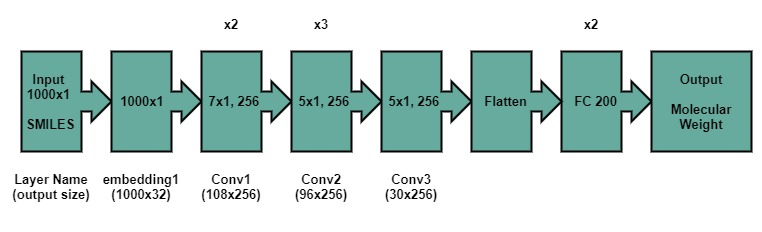
\includegraphics[width=0.5\textwidth]{figures/MW-model_arquitecture.jpg}
        \caption{The architecture of the model that predicts the molecular weight of a compound based on its SMILES string.}
        \label{fig:mw-architecture}
    \end{figure}
    \begin{figure}
        \centering
        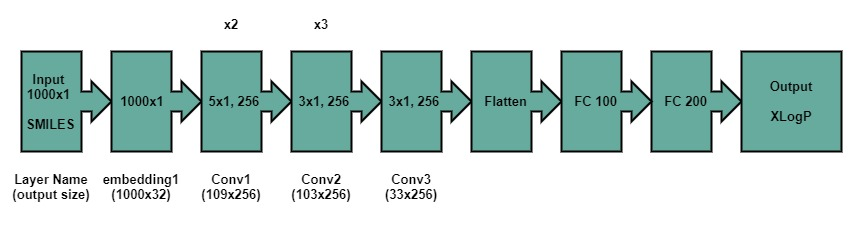
\includegraphics[width=0.5\textwidth]{figures/XLogP-model_arquitecture.jpg}
        \caption{The architecture of the model that predicts the XLogP of a compound based on its SMILES string.}
        \label{fig:xlogp-archi1}
    \end{figure}
    \begin{figure}
        \centering
        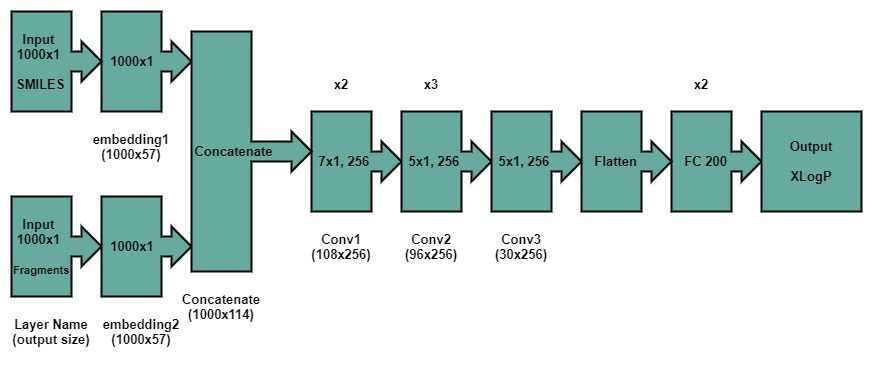
\includegraphics[width=0.5\textwidth]{figures/XLogP_frag_model_arquitecture.jpg}
        \caption{The architecture of the model that predicts the XLogP of a compound based on its SMILES string and RECAP fragments.}
        \label{fig:xlogp-archi2}
    \end{figure}